\subsubsection{18.11.14}

\begin{enumerate}
	\item Время начала и окончания собрания:
	16:00 - 1:00
	\item Цели собрания:
	\begin{enumerate}
	  \item Потренироваться в управлении роботом.
	  
    \end{enumerate}
	\item Проделанная работа:
	\begin{enumerate}
	  \item Первые же испытания показали несостоятельность идеи установки внутрь трубы ковша пластмассовых вставок из бутылок, поскольку это значительно сокращало внутренний диаметр трубы и в случае, когда одноваременно захватывалось несколько мячей, они мешали друг другу проходить по трубе. Для более стабильного выкатывания шариков из ковша было решено демонтировать обрезки от пластиковых бутылок и оставить каркас из металлической сетки. Это устранило возникшую проблему, однако теперь у трубы не хватало длины для закидывания мячей в корзины.
      
      \item В процессе тренировок было обнаружено, что сервопривод, опрокидывающий ковш, не способен повернуть его, когда он заполнен мячами. Для исправления этого на заднюю часть ковша был установлен противовес в виде рыболовного груза массой около 100 г.
      
      \begin{figure}[H]
      	\begin{minipage}[h]{0.2\linewidth}
      		\center   
      	\end{minipage}
      	\hfill
      	\begin{minipage}[h]{0.27\linewidth}
     	 	 \center{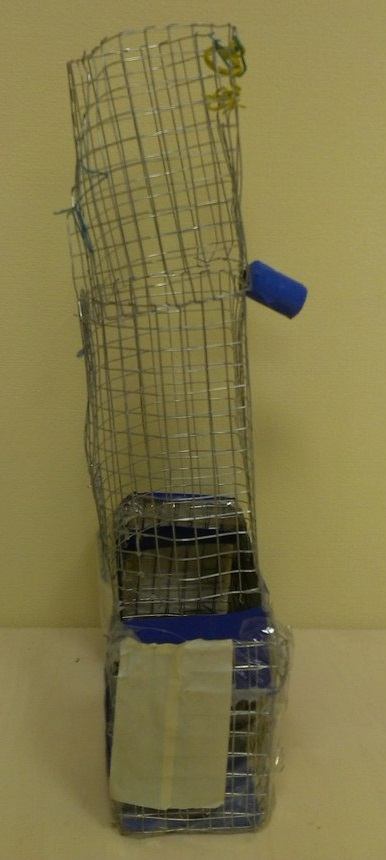
\includegraphics[scale=0.2]{days/18.11.14/images/01}}  
      	\end{minipage}
      	\hfill
      	\begin{minipage}[h]{0.27\linewidth}
      		\center{
\includegraphics[scale=0.18]{days/18.11.14/images/02}}
      	\end{minipage}
      	\hfill
      	\begin{minipage}[h]{0.2\linewidth}
      		\center  
      	\end{minipage}
      	\caption{Противовес на ковше}
      \end{figure}
      
      \item Также было обнаружено, что 2 привода не справляются с раздвиганием подъемника, из-за чего предохранители нагреваются и размыкают цепь, лишая оператора возможности управлять подъемником. Для уменьшения нагрузки на приводы была установлена понижающая передача с соотношением 1:2.
      
     % \begin{figure}[H]
     % 	\begin{minipage}[h]{0.2\linewidth}
     % 		\center  
     % 	\end{minipage}
     % 	\begin{minipage}[h]{0.6\linewidth}
     % 		\center{
\includegraphics[scale=0.3]{days/18.11.14/images/03}}
     % 		\caption{Механизм лебедки с передаточным отношением 1:2}
     % 	\end{minipage}
     % \end{figure}
      
      \item После установки передточного отношения моторы стали справляться с раздвиганием подъемника, однако в некоторых случаях подъемник заклинивало. Связано это с тем, что в какой-то момент ремень начинает зажимать между верхней поперечной осью самой нижней рейки и нижней осью второй рейки. Во избежание этого нужно поставить ограничители, которые не будут позволять нижней оси второй рейки подниматься слишком высоко.
          
    \end{enumerate}
    
	\item Итоги собрания: 
	\begin{enumerate}
	  \item Пластмассовые вставки убраны с трубы ковша. 
	  
      \item На моторы, раздвигающие подъемник, установлена понижающая передача с соотношением 1:2.
      
      \item Для нормальной работы системы опрокидывания ковша на ковш был установлен противовес.
    \end{enumerate}
    
	\item Задачи для последующих собраний:
	\begin{enumerate}
	  \item Установить ограничители движения оси на подъемнике.
	  
	  \item Удлиннить трубу ковша, чтобы можно было закидывать мячи в подвижные корзины.
	  
	  \item Продолжить тренироваться в управлении роботом.

    \end{enumerate}     
\end{enumerate}
\fillpage